\chapter{Introduction}
\label{chap:intro}

%%%%%%%%%%%%%%%%%%%%%%%%%%%%%%%%%%%%%%%%%%%%%%%%%%%%%%%%%%%%%%%%%%%%%%%%%%%%%%%%%%

Here the ideas discussed in this dissertation are contextualized. Giving this, a brief introduction, some definitions and main variants to the Timetabling Problem (TTP) are provided.

% ------------------------------------------------------------
\section{Introducing the basic timetabling problem}

Timetabling problems are a kind of practical scheduling challenge faced by many organizations and important for their daily operations to succeed. Application areas vary widely from sport event timetabling to nurse scheduling, lectures scheduling and transportation timetabling. The general problem can be described as needing to satisfy a set of demands through the scheduling of meetings between those who demand and the available resources. The resulting timetables must be feasible and acceptable to all people and resources involved.

This work is about timetabling in the school environment, which is where the original problem was set.

In school timetabling, a given number of lectures, involving students, teachers and classrooms, should be schedule over a fixed period of time (typically a week), while usually having to satisfy a set of additional constraints of various types. For an actual and applied purpose, besides mandatory operational constraints, such as avoiding resources overbooking, it is essential to consider several solution quality constraints, which can be related to institution, pedagogical and personal needs.

Because schools differ a lot in their educational policies, both when considering the same country and especially more between distinct countries, the criteria for quality and even timetable feasibility definition also depends on each educational system. Here the Brazilian school educational system is embraced. Studies based on the German school system can be found at \cite{Michael2002}, on the Greek system at \cite{Birbas1997} and \cite{Birbas2009}, on Brazilian system at \cite{Haroldo2012}. An overview of school timetabling research is provided by \cite{SchoolOverview2010}, describing the most common operational and quality requirements and the different solving methods that have been used.

University timetabling problems have also been very studied and have many similarities with the school version. Studies based on a Turkish university system can be found at \cite{Guenalay2006} and on a Greek university system at \cite{Daskalaki2005}. For more complete approaches, one can check at \cite{Carter2001} for a Canada university system and at \cite{Murray2007} for an American university system.

The problem is known to be a hard problem and therefore many researchers have shown an interest in it since the early 1960's. Schaerf \cite{Schaerf99} showed that the school timetabling problem is NP-complete and that exact optimal solution could be obtained only for small size problems. Furthermore, enhancing a model with real-world practical and quality requirements increases even more the complexity of the problem. For instance, considering the compactness requirement for students timetables (see ~\ref{constrStudentGap}), \cite{Asratian2002} shows that deciding whether a timetable that guarantees compactness for the students exits is NP-complete by itself.



% ------------------------------------------------------------
\section{Brazilian school timetabling problem}

In Brazil, basic educational system is split in 3 stages:
\begin{enumerate}
\item Fundamental Education I
\item Fundamental Education II
\item Upper secondary education
\end{enumerate}

Fundamental Education is mandatory for children ages $6-14$. There are 9 \q{years} (as opposed to the former 8 \q{grades}). The current \q{First Year} broadly corresponds to the former Pre-School last year of private institutions, and its aim is to achieve literacy. Generally speaking, the only prerequisite for enrolling in first year is that a child should be 6 years old.

The Federal Council of Education establishes a core curriculum consisting of Portuguese language, history, geography, science, mathematics, arts and physical education (for years 2, 3, 4 and 5). As for years 6, 7, 8 and 9, one or two foreign languages are also compulsory (usually an English and optional language).

Each education system supplements this core curriculum with a diversified curriculum defined by the needs of the region and the abilities of individual students.

Fundamental Education is divided in two stages, called \q{Ensino Fundamental I} (years $1-5$) and \q{Ensino Fundamental II} (years $6-9$). During \q{Ensino Fundamental I} each group of students is usually assisted by a single teacher. As for \q{Ensino Fundamental II}, there are as many teachers as subjects.

Public fundamental schools are funded by municipal and state governments. The education is similar to the British.

Students must have finished their Fundamental education before they are allowed to enroll in Secondary education (\q{Ensino M\'{e}dio}), which takes 3 years. Secondary education core curriculum comprises Portuguese (including Portuguese language, Brazilian and Portuguese literature), foreign language (usually English, also Spanish and very rarely French today), History, Geography, Mathematics, Physics, Chemistry and Biology. Philosophy and Sociology, which were banned during the military dictatorship (1964 to 1985), became compulsory again. The courses provided during this period are essentially designed to allow a young person to enter into an university. A minority of schools provides professional training along with mainstream secondary education. Professional training courses usually last 2 years and can be taken during the 2nd and 3rd years of Secondary education.

Public middle schools are provided by state governments.

Once a student has successfully completed secondary education, they may continue their studies at a public or private university. To enter a public university, students must sit an entrance exam, known as \q{vestibular}. Entrance exams to a private university are often little more than a formality and, as a consequence, public university degrees are usually valued much more highly than those from private institutions.

The normal practice in Brazilian schools, both public and private, is to mix students of all study directions together in the same class. Due to the entrance exam to universities, it is common though at private schools for students at last year of secondary education to have extra specialized classes, which depend on their choice for undergraduation course.

Data from \cite{WikiEducationInBrazil}.


% ------------------------------------------------------------
\section{Practical and realistic formulation}

Both school and university timetabling problems have been studied for over 50 years now. Many potentially useful solving algorithms and techniques have been discussed and offered, but unfortunately much of the work in this area has been conducted using artificial data sets or based on greatly simplified versions of actual problems. Often the considered scenario has already preassigned sets of entities, like professors to classes in the case of school timetabling or students to course sections in the case of university. Besides, methods developed have most times been restricted to a single university department or school block, instead of being extended to the solution of actual university and school problems of any large scale. Whenever the different departments or blocks have dependencies, like sharing resources, usually teaching staff, such partition of the problem is relevant and can therefore be prejudicial to the final solution quality and acceptance.

For the university environment, we draw attention to \cite{Carter2001} and \cite{Murray2007} as those who made efforts on solving very realistic versions of the problem for universities in Canada and in USA. They described both the methods used for solving the problems and the challenges faced during the process of deploying solutions.

The major differences between many of the problems studied and their real life counterparts are the additional complexity imposed by course structures, the variety of constraints imposed, and the distributed responsibility for information needed to solve such problems at a university-wide level.

As pointed out in \cite{Murray2007}, the biggest obstacle to solve actual university course timetabling problems is that the complexity can increase considerably beyond that represented in standard formulations of the problem. As the complexity increases, it is easy to be caught in the dual bind that the problem is both more challenging to develop an effective solution approach for, and this approach is less likely to be usable on other university timetabling problems. Every institution has its own particularities, which make it harder to build a single and general solver for multiple institutions.

As observed by Carter \cite{Carter2001}, there are few published papers that described actual implementations of course timetabling. From what we know, the first example of an automated and integrated course timetabling and student scheduling system across a institution was developed for the University of Waterloo between 1979 and 1985. Although the system was implemented 29 years ago, much of the discussion is still very relevant. By 2001, Carter expressed at \cite{Carter2001} his belief that there was still no system for solving the large-scale course timetabling problem with such level of mathematical sophistication.

By 2006, Guenalay and Sahin introduced at \cite{Guenalay2006} a Decision Support System (DSS) for the university timetabling that allows the direct involvement of the decision maker. They affirmed that their model was the first one which simultaneously combined such a DSS approach with a goal programming optimization tool.

At \cite{Unitime} the Unitime software is described and widely documented. It is an open source system used at Purdue University and is also the focus of \cite{Murray2007}.
\fixme{citar mais software!}


% ------------------------------------------------------------
\section{Main similar formulations and their differences}

For solving the high school timetabling problem, this work is based on an integer programming formulation together with strategies for helping at the convergence in the best solution search process.

Among the existing published works that considered more realistic formulations for high school timetabling problems, we highlight \cite{Birbas2009} and \cite{Birbas2009} as those whose embraced problems were the most similar to the one considered in this work. Several practical issues emphasized by them were also identified during TRIEDA's development and were referenced along this work.

Still, there are differences between their timetabling problems and the one here presented. Following, the major points are listed.
-
-
-

Further differences can be identified along this work.

Because TRIEDA is a commercial software, it has been developed to be as portable and flexible as possible. Particularly, the system embraces most common rules and cases found in Brazilian universities and schools.


% ------------------------------------------------------------
\section{Data accuracy and Politics}

\mynotes{from \cite{Murray2007}}
Since timetabling is a resource allocation problem, at most big educational institutions responsibility for constructing the timetable is distributed among the academic units with the faculty, physical facilities, and other resources required for offering instruction. Murray, M\"{u}ller and Rudov\'{a} observe at \cite{Murray2007} that providing support for this distributed responsibility is important because departmental timetablers have a much more intimate knowledge of the needs of the courses offered, the professor who might be able to teach a particular class, and the spaces available for specialized instruction than any database that might be maintained centrally. Maintaining each department's sense of ownership in the timetables that are produced is also an important factor in their acceptance of the solutions produced by an automated timetabling process. They say the process needs to be one that assists them rather than replaces them.

Obtaining coherent and correct data is a particular important and sensitive issue. Because data accuracy depends on each department, it is extremely important that data collection phase of an automating process has a deep involvement of all of those who usually operate in the traditional manual process. Any inaccuracy of data can result in a bad or even non-deployable solution.

\fixme{citar funcionalidade: motivos de nao atendimento}

Murray, M\"{u}ller and Rudov\'{a} tells at \cite{Murray2007} that inequity in the quality of time and room assignments received by different departments and faculty members doomed a previous attempt at automating the timetabling process at Purdue University. A similar situation was faced by TRIEDA in July of 2014 while an attempt of deploying a solution in a Brazilian university.

Automating people assignments is different from automating other process --- the optimization factor is definitely \textbf{not} more important than people satisfaction. Only keeping that in mind it is possible to obtain an actual deployable solution.

As wisely pointed out in \cite{Carter2001}, practical course timetabling is 10\% graph theory, and 90\% politics. Carter tells that when they first began designing a timetabling system for University of Waterloo, they were warned that they can not dictate when professors will teach courses. Consequently, they were told that course timetabling could not work or, more precisely, that they can not assume that the timetable can use a clear slate. This is because part-time professors may be available only on certain and specific days or times. University professors often have other commitments and industrial research projects. Teaching is only a part of their job, and probably less than half of their time is devoted to teaching. Similar statement is valid for high school teachers. It is very common that they teach in more than one school or have other activities.

It follows that it is essential to allow professors to restrict their available timetables as much as they want.

Guenalay and Sahin describe at \cite{Guenalay2006} an approach for university timetabling with a goal programming optimization tool in order to process the instructor teaching time preferences. As they observed, using a multi-objective function for considering instructor available preferences may not be enough for ensure a reliable and acceptable solution.

Professors' availabilities and preferences issue should therefore not be underestimated.

The primary design goal is not necessarily finding a true optimal solution, but to assist academic timetablers with the problem of building a good and better timetable in an efficient way.


% ------------------------------------------------------------
\section{Timetabling Groups and Conferences}

% ---------------
\subsection{Practice and Theory of Automated Timetabling Conferences (Patat)}
\label{patat}

\begin{figure}[h]
\hfill
\includegraphics[scale=0.8]{figures/patat.png}
\end{figure}

The International Series of Conferences on the Practice and Theory of Automated Timetabling (PATAT) is held biennially as a forum for both researchers and practitioners of timetabling to exchange ideas. The first edition was held in Edinburgh (UK) in 1995, and since that editions have taken place in Canada, Germany, Belgium, USA, Czech Republic, Northern Ireland and Norway. See \cite{Patat}.

Whether it is sporting events, educational institutions, transportation or employee management the construction of efficient timetables which provide the maximum in way of flexibility for all constituent parts is as important as it is challenging. An increasingly important aspect within organizations is an automated approach which maximizes all aspects of resource usage. In doing so a number of quantitative and qualitative challenges must be dealt with from both a technical and practical perspective.

An important aim of the Conference is to align the needs of practitioners and the objectives of researchers. This is achieved through the presentation and application of leading edge research techniques. Practitioners and Researchers alike are encouraged to present their work and experiences through a number of key presentations and workshops with the overall goal of developing efficient and practical solutions.

The link between planning and management within the educational sector is explored and keynote talks are delivered by leading practitioners from the University sector and those companies which provide automated timetable solutions.


% ---------------
\subsection{International Timetabling Competition (ITC)}
\label{itc}

\begin{figure}[h]
\hfill
\includegraphics[scale=0.8]{figures/itc.png}
\end{figure}

The International Timetabling Competition (ITC) has happened in 3 editions, in 2002, 2007 and 2011.

Not much information was found about the first ITC, in 2002.

The second International Timetabling Competition, in 2007, focused on examination and courses timetabling problems and was sponsored by PATAT and WATT (see \cite{ITC2007}).

The third International Timetabling Competition, in 2011, was devoted to High School Timetabling and sponsored by PATAT, EventMAP and CTIT (see \cite{ITC2011}).

The competition aims to stimulate timetabling research generally, and especially to encourage the alignment of research with practice by offering real-world instances of timetabling problems for solution. The overall objectives are the following:
\begin{itemize}
\item Allow researchers to trial their techniques in a competitive setting on 'real world' practical problems.
\item Close the gap which currently exists between research and practice within this important area of operational research.
\item Encourage research in the area of complex NP hard real world problems.
\item Attract researchers from all disciplines to compete.
\item Further algorithmic development in the area of educational development.
\item Generate all-time best solutions to these problem instances.
\end{itemize}

Although for the sake of the competitive element not all aspects of the real world problem are included, more depth and complexity have been introduced significantly at each new edition.

The competition is composed of three separate rounds. Although there is much overlap, these rounds represent distinct problems within the area of educational timetabling both from a research and practical perspective.

The first round made use of a set of existing benchmark data and aims at generating the best recorded results. Competitors can use what ever resources and techniques in attempting to generate their solutions. This is an attempt to replicate the 'real world' where timetablers are more interested in achieving the 'best' solution as opposed to getting a solution quickly.

The second round makes use of the hidden archive. The winner is chosen based on effectiveness in a specified time on these instances. Imposing a restrictive time limit allows for the investigation of algorithmic techniques which can provide 'good' solutions in a short space of time. This is often a key requirement in the 'real world' when alternative solutions are required in a short space of time. Hidden instances are used to ensure submitted techniques are not overly tuned to particular instances of the data.

In the third round, the hidden archive instances are released. As with the first round, competitors can use what ever resources and techniques in attempting to generate their solutions. Solutions are to be submitted one month later.

All instances are provided in XML.


% ---------------
\subsection{Data sets and an input format for High School Timetabling (Hstt)}
\label{hstt}
% Benchmarking project for highschool

The research in (High) School Timetabling was lacking the availability of exchangeable benchmarks in a uniform format. For this reason a group of researchers agreed on an xml-standard to exchange their datasets. Latest update says there are around 50 datasets available. This project was reported in the PATAT conferences of 2008 and 2010.

Available are archives and datasets in XHSTT format, an evaluator for instances (by Jeff Kingston) and solutions in XHSTT, and a classification (by Nelishia Pillay) of high school timetabling.

At chapter ~\ref{chap:converting} an attempt for solving XHSTT instances provided by \cite{Hstt} is detailed and registered.

More information about this project at \cite{Hstt}.


% ---------------
\subsection{Ectt}
\label{ectt}
% Udine, Italy

\begin{figure}[h]
\hfill
\includegraphics[scale=0.4]{figures/ectt.png}
\end{figure}

Following the spirit of the International Timetabling Competition (~\ref{itc}), \cite{Ectt} provides a portfolio of formulations for the Curriculum-Based Course Timetabling problem as defined in [Bonutti, De Cesco, Di Gaspero and Schaerf, Annals of Operations Research].

Through the website it is possible to download instances (both in text-only and XML format) and solutions contributed from the research community; validate your solutions online or download the source code of a solution validator; insert solutions, lower bounds, instances, and links of interest for the community; and generate random instances. All problem instances available to download are based on real data from various universities.


% ---------------
\subsection{Research Group on Scheduling and Timetabling in Udine}
\label{satt}

\begin{figure}[h]
\hfill
\includegraphics[scale=0.7]{figures/satt.png}
\end{figure}

The Scheduling and Timetabling research group in Udine is working on the solution of scheduling problems using both local search techniques and their hybridization with other paradigms (e.g. constraint programming). The researchers involved in the group have developed both academic prototypes and production systems for the solution of practical scheduling problems, such as workforce scheduling, shift design, timetabling, and sport scheduling. In addition, the group has been active in the system-modeling side, in the development of languages and tools for specifying problems and applications.

Among the several projects to which the group is involved, we highlight the following for being related to timetabling problems:
\begin{itemize}
\item Educational Timetabling
The educational timetabling problem consists in scheduling a sequence of events (typically lectures or examinations) which involves teachers and students in a prefixed period of time, satisfying a set of constraints of various types. Constraints involve, among others, overlapping of events with common participants, capacity of rooms, and student and teacher workload.
\item Healthcare
The Patient Admission Scheduling Problem (PAS) consists assigning patients to beds in such a way to maximize both medical treatment effectiveness and patients' comfort. The Dynamic Patient Admission Scheduling Problem under Uncertainty (PASU) extends the PAS problem, by including several real-world features, such as the presence of emergency patients, uncertainty in stay lengths, and the possibility to delay admissions.
\item Multi-Agent Distributed Timetabling
TT-MAS is a multi-agent system for distributed course timetabling. It is considered the timetabling problem for a set of university departments, in which each department prepares the schedule according to private rules, constraints, and objectives, and relying on own resources. In order to share and/or exchange resources for mutual benefits the system allows the departments to negotiate on a common marketplace and making use of an artificial currency.
\end{itemize}

More info at \cite{UdineSATT}.


% ---------------
\subsection{EURO Working Group on Automated Timetabling (WATT)}
\label{watt}

\begin{figure}[h]
\hfill
\includegraphics[scale=0.7]{figures/euro.png}
\hfill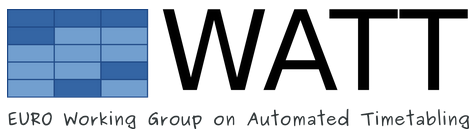
\includegraphics[scale=0.35]{figures/watt.png}
\end{figure}

WATT is the EURO Working Group on Automated Timetabling, formed to discuss, promote, and perform research into automated timetabling problems and methods.

The WATT community was launched in the wake of the first international conference on the Practice and Theory of Automated Timetabling in 1995 (PATAT'95). Ever since, the interest group has flourished and memberships have steadily increased.

The main studied categories are:
\begin{itemize}
\item Employee timetabling, which consists of \q{Nurse rostering} and \q{Personel scheduling};
\item Educational timetabling, which consists of \q{Course timetabling}, \q{University timetabling} and \q{Exam timetabling};
\item Sports timetabling, which consists of \q{Tournament scheduling} and \q{Referee assignment};
\item Other timetabling problems.
\end{itemize}
Each category provides reference datasets and references to literature on the respective timetabling subject.

Further information at \cite{Watt}.


% ---------------
\subsection{Mista: Multidisciplinary International Scheduling Conference}
\label{mista}

\begin{figure}[h]
\hfill
\includegraphics[scale=0.7]{figures/mista.png}
\end{figure}

Mista is a conference series which serves as a forum for an international community of researchers, practitioners and vendors on all aspects of multi-disciplinary scheduling. The aim is to bring together scheduling researchers and practitioners from all the disciplines that engage with scheduling research. 

It was held biennially since 2003 alternating between cities in UK, USA, France, Ireland and Belgium. In August 2015 the seventh conference will be held in Prague, Czech Republic.

Further information at \cite{Mista}.

% ------------------------------------------------------------

This is a test reference to \cite{Carter2001}.    % Waterloo, Canada
This is a test reference to \cite{Murray2007}.    % Purdue (unitime), USA
This is a test reference to \cite{Unitime}.       % website
This is a test reference to \cite{DSS}.           % website
This is a test reference to \cite{Guenalay2006}.  % Bilkent, Turkey, (DSS)
This is a test reference to \cite{Schaerf99}.  		% Schaerf99
This is a test reference to \cite{Michael2002}.   % Michael2002
This is a test reference to \cite{SchoolOverview2010}.   % SchoolOverview2010
This is a test reference to \cite{Birbas2009}.    % Birbas2009
This is a test reference to \cite{Mimosasoftware}.
This is a test reference to \cite{Eventmap}.




%%%%%%%%%%%%%%%%%%%%%%%%%%%%%%%%%%%%%%%%%%%%%%%%%%%%%%%%%%%%%%%%%%%%%%%%%%%%%%%%%%

\section{Dissertation Outline}
This work is organized as follows: 
\begin{itemize}
	\item Chapter ~\ref{chap:timetabling} introduces Trieda's timetabling problem.
	\item Chapter ~\ref{chap:mipformulation} shows the mathematical formulation for the problem.
	\item Chapter ~\ref{chap:strategies} presents different approaches and strategies for solving the MIP formulation.
	\item Chapter ~\ref{chap:constranalysis} analyzes the impact of some requirements in the MIP solving.
	\item Chapter ~\ref{chap:converting} presents an attempt to converting a XHSTT format into a Trieda's problem format.
	\item Chapter ~\ref{chap:conclusions} contains the conclusions of this work.
\end{itemize}